\textbf{COLUNI 2019 -- Questão 34}\par\medskip Analise o mapa abaixo:

\par

\textbf{Comércio Mundial por grandes regiões}

\par

(Fonte: FERREIRA, Graça Maria Lemos. \textbf{Atlas Geográfico}: espaço mundial. São Paulo: Moderna, 2013, p. 51.)

\par

De acordo com as informações do mapa, assinale a afirmativa INCORRETA:

% COLUNI-AUTO-FIGURES-BEGIN
\begin{figure}[htbp]
\centering
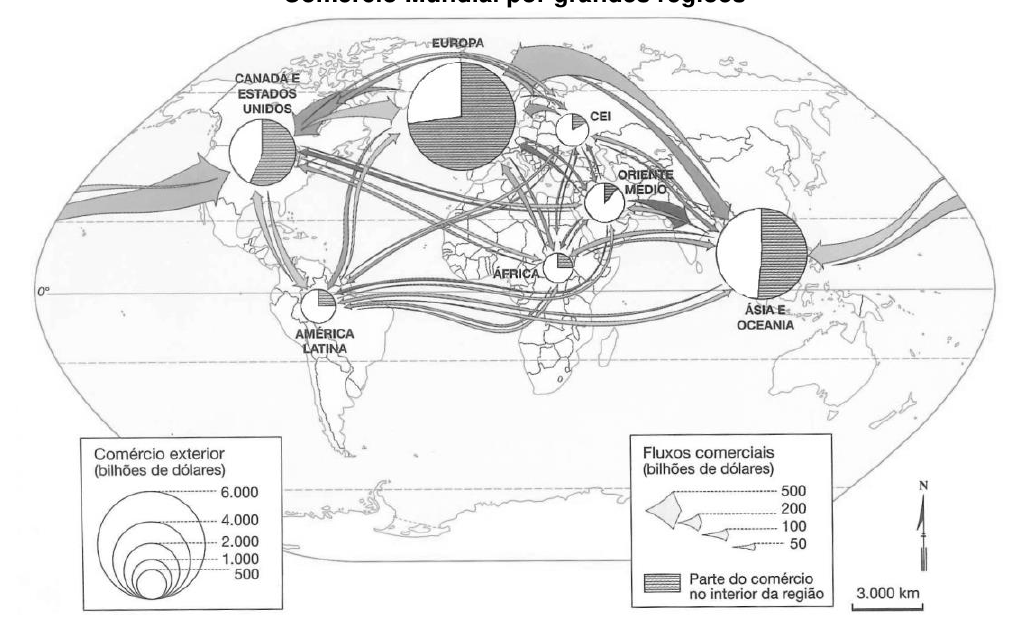
\includegraphics[width=0.95\linewidth]{static/simulados/coluni/figuras/2019/questao-34/figura-1.png}
\end{figure}
% COLUNI-AUTO-FIGURES-END
\begin{enumerate}
\item A Europa tem mais da metade dos fluxos comerciais voltados para o mercado interno.
\item A América Latina possui grande número de transações comerciais internas.
\item A Europa e a Ásia juntas são responsáveis por mais fluxos comerciais que as demais áreas do globo.
\item Os países subdesenvolvidos têm maior participação no comércio externo do que interno.
\end{enumerate}
